\section{Эксперемент}
\begin{eqnarray} 
    FeSO_4 \cdot (NH_4)_2SO_4\cdot 6H_2O + 
    NaOH \xrightarrow{} 
    2NH_3 &\uparrow + Fe(OH)_2 \downarrow + 
    2Na_2SO_4 + 8H_2O \\
    MnSO_4 + NaOH &\xrightarrow{} 
    Mn(OH)_2 + Na2SO_4 \downarrow
\end{eqnarray} 

\begin{center}
    \begin{tabular}{l||l||l}
        Compound & Color & Transparency \\ \hline \hline
        $Fe(OH)_2$ & Темно-зеленый &    Непрозрачный \\
        $PbS$ & Золотисный-оранжеый &    Непрозрачный 
    \end{tabular}
\end{center}

\begin{figure}[h]
    \centering
    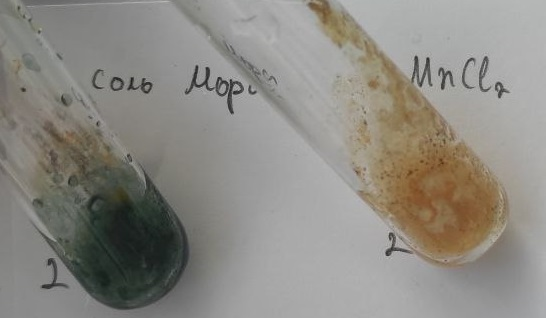
\includegraphics[width=1\linewidth]{Ex_2/1.jpg}
     \caption{}
    \label{ex_2_1}
\end{figure}

